\section{Overview of Our Approach}
\label{sec:overview}


In this section, we provide an overview of our approach \name and introduce \emph{\nameenclave{}s}. \Nameenclave{}s dynamically extend the TCB of traditional TEEs running on the CPU to the \sphw. \Nameenclave{}s consist of multiple distributed enclaves that run on various hardware components such as the CPU and \sphw as shown in Figure~\ref{fig:new_system}. \Nameenclave{}s aim to provide similar security properties as traditional enclaves, such as integrity, attestation, and data isolation from other enclaves and the attacker-controlled OS. 

\begin{figure}[tbp]
    \centering
    %Source:
    %https://drive.google.com/file/d/1K8Jg0eXF1W2dpIVLmvP8D0k-qK-dHq4P/view?usp=sharing
    %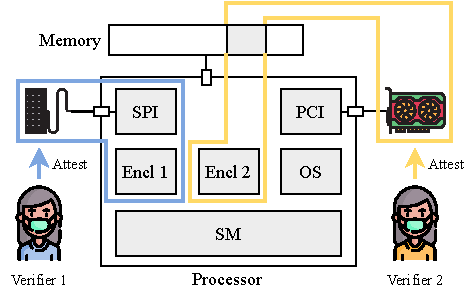
\includegraphics[width=0.7\linewidth]{chapters/PIE/images/cpu_bus_peripheral-Page-4.pdf}
        %   \includestandalone[width=\linewidth]{images/tikz/new_system}
	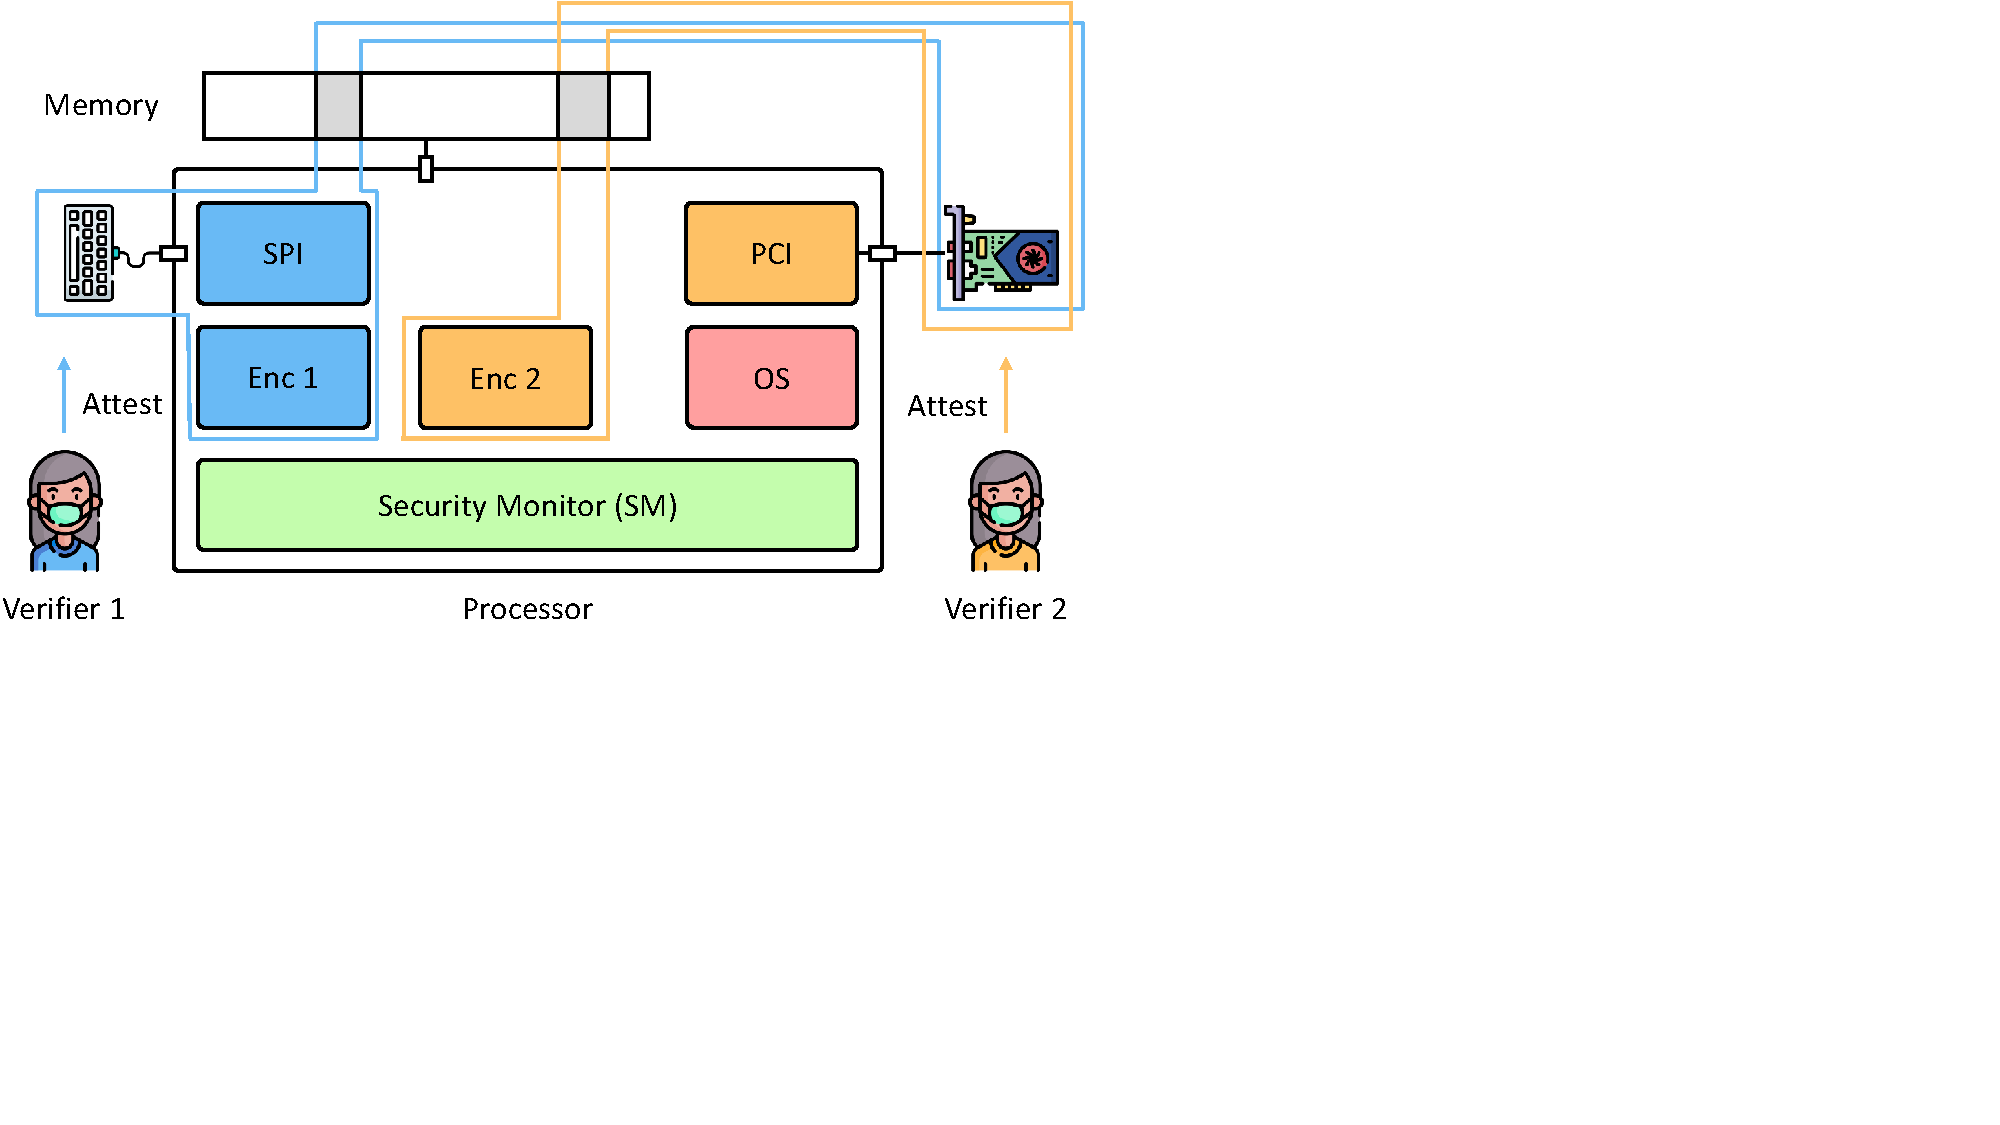
\includegraphics[trim={0 8cm 15cm 0}, clip, width=\linewidth]{chapters/PIE/images/pwe_idea.pdf}
    \caption[\Nameenclave{}s consists of different applications and \sphw]{Two \nameenclave{}s are highlighted by blue and yellow outlines. The blue one consists of \texttt{Encl1}, a keyboard that is connected over the memory-mapped SPI bus and a GPU connected over PCI through DMA. This case represents a trusted path scenario where user requires both input and output. The second consists of \texttt{Encl2} and a GPU connected over PCI through DMA. The second one represents a usecase such as executing machine learning workload in the GPU cores.}
    \label{fig:new_system}
\end{figure}



\subsection{Enclaves within a \nameenclave}
\label{sec:overview:enclaves}

A \nameenclave{} consists of multiple enclaves that run on different hardware components and securely communicate with each other. A \nameenclave{} typically contains several interconnected processor-local enclaves and \sphw enclaves. In the following, we describe the two main enclave types that form a \nameenclave{}.

\myparagraph{Processor-local enclaves}
\label{sec:overview:enclaves:processorEnclave}

Processor-local enclaves are equivalent to traditional enclaves and their runtime memory must be isolated from the OS and should only be accessible to the enclave itself. To achieve that, we use physical memory protection (PMP) from the RISC-V privilege standard~\cite{riscv2019privspec} as introduced by Keystone.

We further differentiate two types of processor-local enclaves: \app{}s, and \ce{}s which encapsulate the application-specific, and driver logic, respectively. As seen in Figure~\ref{fig:sharedMemory}, $AE_1$, and $CE_1$ are the \app, and \ce in the blue-outlined \nameenclave of Figure~\ref{fig:new_system}. The \ce also provides isolation between the \apps in a scenario where multiple \apps want to access a certain \sphw. Therefore, \ce enforces access control on the connected \apps in terms of how a certain \sphw can be accessed, e.g., exclusive access to a keyboard or shared concurrent access to a GPU. 
% $AE_1$ uses $CE_1$ to communicate with $P_1$ that is a \sphw enclave which we discuss in the following. 

\myparagraph{Enclaves on \sphw}
\label{sec:overview:enclaves:peripheralEnclave}
Most \sphw run some firmware or even some custom code (e.g., graphic shaders) which has to be included in the TCB of a \nameenclave.
E.g., the GPU and its firmware in Figure~\ref{fig:new_system} is part of the yellow \nameenclave. Since a remote verifier also wants to attest to the \sphw, they have to be modified to support attestation. However, we stress that these modifications  remain rather small (c.f. \Cref{sec:eval:accel}) and usually only involve small changes in the device firmware. %Essentially, one only has to add a certificate from the manufacturer for a secret key stored in the \sphw.

\begin{figure}[tbp]
     \centering
     %\includestandalone[width=0.9\linewidth]{images/tikz/approach}
     %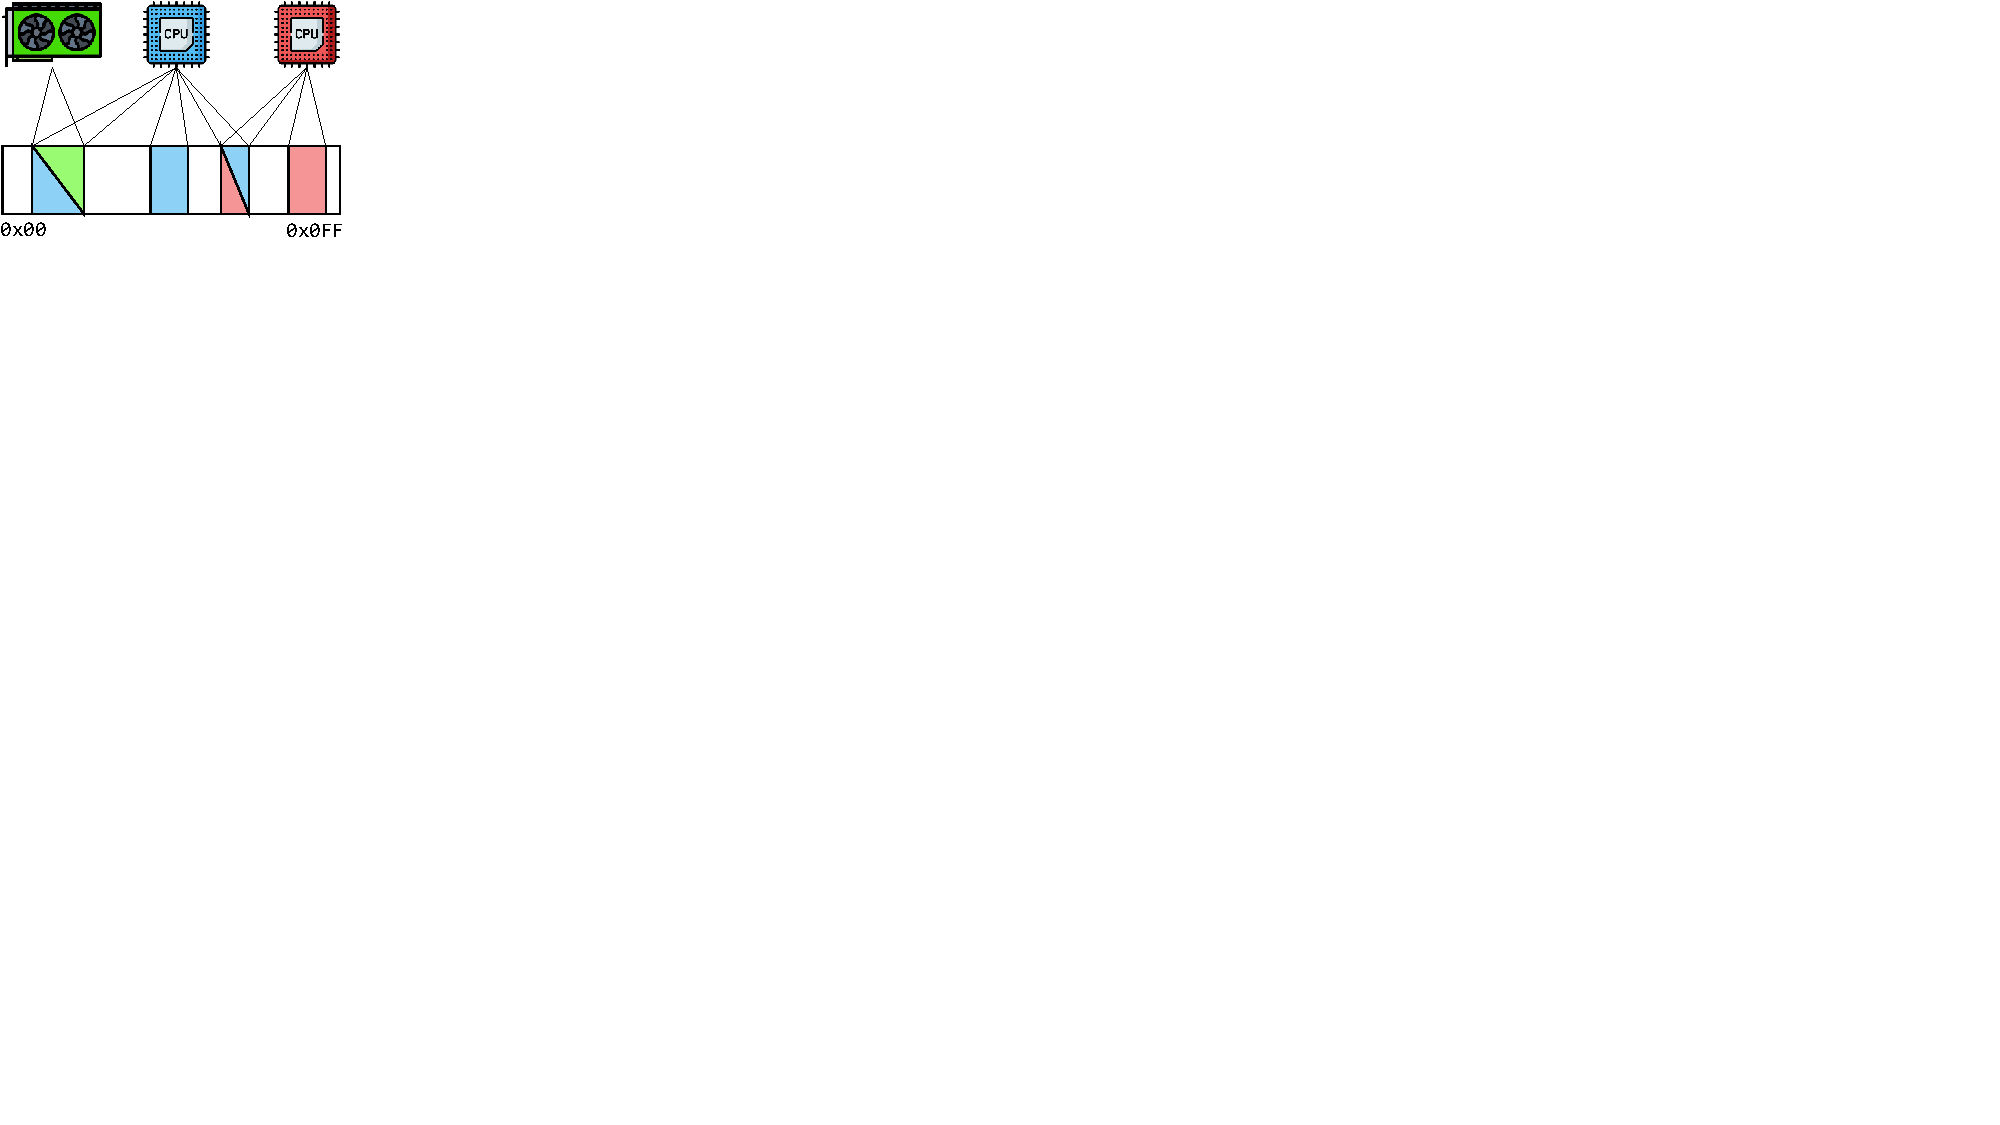
\includegraphics[trim={0 15cm 28cm 0}, clip, width=0.5\linewidth]{approach.pdf}
    %  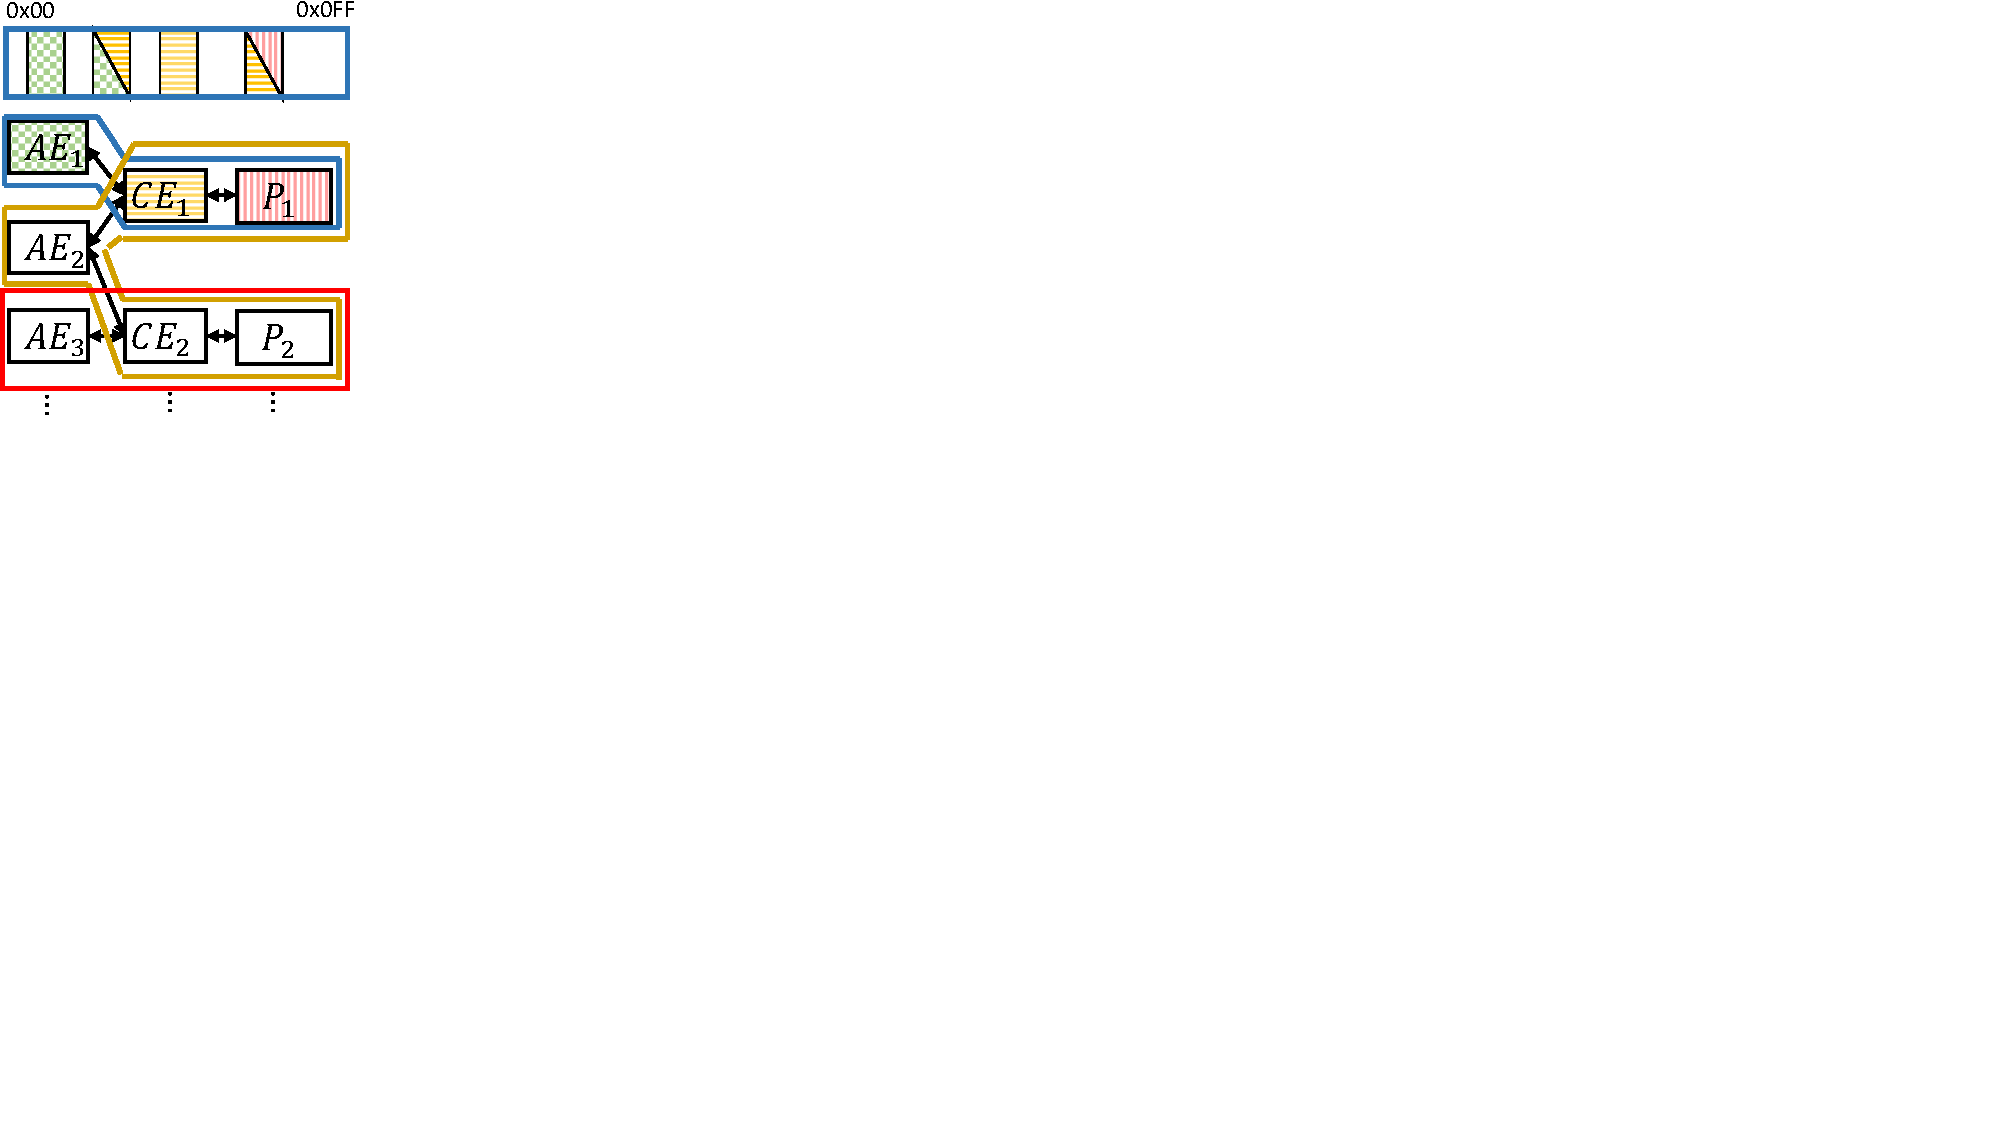
\includegraphics[trim={0 12cm 27cm 0}, clip, width=0.5\linewidth]{approach_combined.pdf}
     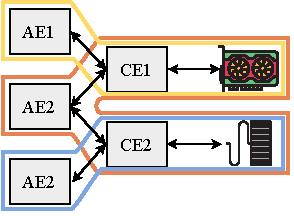
\includegraphics[width=0.4\linewidth]{chapters/PIE/images/softwaredesign.pdf}
     
     %\caption{Example configuration where a red CPU enclave shares some memory with a blue CPU enclave and another shared buffer with a GPU. The solid color memory cells correspond to the private enclave memory regions, and the cells with mixed color denote shared memory regions.}
     \caption[Three example \nameenclave{}s in \name{}'s software design]{Three example \nameenclave{}s in \name{}'s software design with \app{}s (AE), \ce{}s (CE), a GPU, and a keyboard. Note that the red \nameenclave{} is spanning over two external devices and \ce{}s isolate the data from the different \app{}s.}
     \label{fig:sharedMemory}
\end{figure}

\subsection{Communication with \sphw}
\label{sec:approach:comm}

To enable processor-local enclaves and \sphw enclaves to securely communicate, we make the observation that these devices generally communicate over mapped address regions: They either use an address range that is not reflected in DRAM, so-called memory-mapped-input-output registers (MMIO), or a shared DRAM region accessed via direct memory access (DMA). To maximize compatibility with existing drivers and \sphw, we chose not to change this behavior. Instead, we isolate the address regions that are used in this communication. Existing hardware mechanisms like PMP already allow restricting access to a specific address region. Until now, such hardware mechanisms have been predominantly used to restrict memory access, but in our design, they also allow to restrict access to other address regions that are not in the DRAM range\footnote{E.g., DRAM could occupy the address range \texttt{0x8000000 - 0xF0000000}, whereas other \sphw such as UART could reside at \texttt{0x4000000 - 0x4001000}.}. Note that these address regions from \sphw are either i) static, i.e., hardcoded and provided to the SM in the form of a trusted device tree file, or ii) dynamic, i.e., configured at runtime by the SM. In our design, the SM always maintains a complete overview of all such regions and only allows a single enclave to access an address region of a \sphw.

While we made the changes mentioned above to the SM to support \sphw with both MMIO and DMA, they also enable a new way for enclaves to communicate: shared memory. This reflects a major difference to traditional TEEs because until now; most traditional enclaves could only communicate through the untrusted OS\footnote{Concurrent work~\cite{yu2020elasticlave} has also shown how shared memory can improve the performance of enclaves significantly.}. 
% By supporting DMA regions for \sphw, our design also implicitly supports shared memory between enclaves. 
%Figure~\ref{fig:sharedMemory} shows an example shared memory configuration of our design.


\subsection{Changes within a \nameenclave{}}
\label{sec:overview:awareness}

The untrusted OS manages \sphw devices; hence the OS could remap any device or send a reset signal. E.g., a GPU that is handing sensitive data could be shut down by the OS and remapped to a different GPU during runtime. In such a scenario, the enclave should stop sending sensitive data to the GPU until the remote verifier re-attests the new GPU. Hence, the enclave has to react to these external events, i.e., it has to be aware of the platform's state. 
In traditional TEEs, enclaves are self-sufficient isolated entities and are only dependent on themselves. 
Therefore, they can only be in two states: running or stopped. \Nameenclave{}s are more complex since they can contain multiple enclaves, all of which could be running, stopped, or even killed. \Nameenclave{}s have to react correctly upon any of these events to keep the data confidential. We achieve this by expanding the enclave lifecycle and adding two new events: connect and disconnect. The asynchronous nature of these events requires a detailed analysis of the security of the entire system, e.g., a well-timed disconnect could lead to data leaks across shared memory regions. We solve this issue by assigning ownership of the shared memory among the enclaves that are accessing that memory. Upon any external events, if one of the participating enclaves dies, the sole ownership is transferred to the remaining one (more details in \Cref{sec:lifeycle}). Therefore, the components in the \nameenclave are \emph{platform-aware} since they are aware of any change within their ecosystem.


\subsection{Attestation of a \nameenclave{}}

Since a \nameenclave{} consists of multiple distributed enclaves, attestation poses another challenge. Individual attestations to each enclave that make up a \nameenclave{} could be vulnerable to timely manipulations by an adversary to cause time-of-check-to-time-of-use (TOCTOU) issues. To provide a platform-wide attestation, we need to chain attestation reports of all the components of a \nameenclave. This includes the attestation report of the enclaves and \sphw firmware. Attestation of the \sphw firmware is achieved by signing a challenge message with the key embedded in the \sphw (refer to Section~\ref{sec:overview:enclaves:peripheralEnclave}).
The attestation of a \nameenclave{} could either be a one-time attestation that results in a huge chain of reports or individual attestations of all entities that can be combined by the verifier. 
We show that individual attestations provide more flexibility for the verifier and are secure against TOCTOU attacks by adding unique identifiers to enclaves and appending all connected enclaves' IDs to the attestation report.
%% Ivan: I have removed the following cause it adds no value to the discussion at this point 
%Surprisingly, this even remains true when identifiers are reused. 


% The full state of a system is too detailed to be processed every time it changes or to meaningfully assess whether it is safe for a remote stakeholder to provide its data. Therefore, this last challenge requires concretely defining what parts of the state (and state transitions) of a system are relevant for the security of \name{}.

\begin{figure}[tbp]
    \centering
    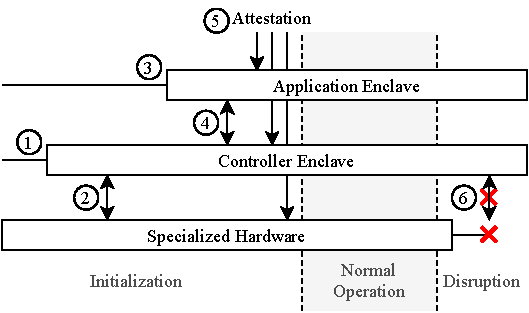
\includegraphics[width=0.8\linewidth]{chapters/PIE/images/cpu_bus_peripheral-Page-5.pdf}
    \caption[Interactions between \nameenclave's components]{An example scenario that illustrates interaction between \nameenclave components.}
    \label{fig:overviewtime}
    % \vspace{-1em}
\end{figure}

\subsection{Summary of Interactions}
To summarize all interactions between the components of a \nameenclave, we present an example scenario in Figure~\ref{fig:overviewtime} with an \app{}, a \ce{}, and a \sphw device. The scenario is as the following:
\begin{enumerate}
    \item[\one] The OS creates and configures the \ce{} and hands over control to the SM. The SM then revokes the OS's access permissions to the private memory regions of the \ce{}.
    \item[\two] The OS requests SM to connect \ce{} with the \sphw device. The SM sets up a new shared memory region and enables access only to the \ce{}.
    \item[\three] Similar to the \ce, the OS creates and configures the \app{}, and then, once again, the SM revokes access to the private memory of the enclave.
    \item[\four] The OS calls the SM to establish a shared memory region between the \ce and the \app. 
    \item[\five] After a remote verifier attests to all enclaves (using the \app as the entry point), sensitive data can be transmitted, and the normal operation starts.
    \item[\six] Any disruption, i.e., a disconnection of the \sphw device, leads to an asynchronous disconnect, where the sole ownership of the shared memory between the device and the \ce{} moves to \ce(see Section~\ref{sec:lifeycle}). Moreover, the enclaves may halt execution until re-attested.
\end{enumerate}

% \subsection{Software Design}

% The last major challenge is to make \name easy to adapt for existing software and \sphw (refer to challenge \emph{d} in Section~\ref{sec:problemStatement:challenges}). A \nameenclave{} must include the driver for any \sphw that it wants to use. However, one big monolithic processor-local enclave that contains all drivers has many downsides. First, \sphw are fully reserved by a single processor-local enclave and cannot be shared among multiple enclaves. And second, every other enclave that also wants to use the same \sphw must also include a driver leading to massive code duplication or, even worse, multiple driver implementations for the same \sphw, each with their own vulnerabilities.

% To combat these downsides of a big monolithic processor-local enclave, we propose a modular software design. All the application logic is kept in an enclave that we call \app. And the driver for a single \sphw is moved to an enclave called \ce{}. This allows multiple \app to use the same \sphw and driver concurrently over one \ce{}. However, to enforce the confidentiality of the various enclaves' data, the \ce{} has to isolate the data, adding to the TCB. This design choice reflects a trade-off between code reuse and usability, and a bit of added complexity and TCB. Note that such a software design also has a significant impact on the attestation mechanism. To remotely attest a \nameenclave{}, the user must attest the \app, all the \ce{}s that it is connected to, and all the \sphw that the \ce{}s are accessing.
